\documentclass[12pt,a4paper]{article}
\usepackage{graphicx}
\usepackage{listings}
\usepackage{color}
\usepackage{hyperref}
\usepackage{geometry}
\usepackage{float}
\usepackage{caption}
\usepackage{subcaption}
\usepackage{tabularx}
\usepackage{booktabs}
\usepackage{svg}
\usepackage{hyperref}
\usepackage{url}

\geometry{margin=1in}

% Code listing style
\definecolor{codegreen}{rgb}{0,0.6,0}
\definecolor{codegray}{rgb}{0.5,0.5,0.5}
\definecolor{codepurple}{rgb}{0.58,0,0.82}
\definecolor{backcolour}{rgb}{0.95,0.95,0.92}

\lstdefinestyle{mystyle}{
    backgroundcolor=\color{backcolour},   
    commentstyle=\color{codegreen},
    keywordstyle=\color{magenta},
    numberstyle=\tiny\color{codegray},
    stringstyle=\color{codepurple},
    basicstyle=\ttfamily\footnotesize,
    breakatwhitespace=false,         
    breaklines=true,                 
    captionpos=b,                    
    keepspaces=true,                 
    numbers=left,                    
    numbersep=5pt,                  
    showspaces=false,                
    showstringspaces=false,
    showtabs=false,                  
    tabsize=2
}
\lstset{style=mystyle}

\title{CS256 Class Project Report: FPGA Tetris}

\author{
    Mohammad Alkhalifah \\
    \texttt{mohammad.alkhalifah@kaust.edu.sa}
    \and
    Mustafa Albahrani\thanks{Contributed to the project implementation; however, this report is an individual submission as per he guidelines} \\
    \texttt{mustafa.albahrani@kaust.edu.sa}
}

\date{\today}



\begin{document}

\maketitle
\newpage

\tableofcontents
\newpage

\section{Introduction}

\subsection{What is Tetris?}
Tetris is a tile-matching puzzle game originally designed by Alexey Pajitnov in 1985. The player manipulates falling geometric shapes called \textit{tetrominoes}---each composed of four square blocks---rotating and positioning them to complete horizontal lines on a 10$\times$20 grid. Completed lines are cleared, and the game ends when pieces stack to the top of the playfield.

\subsection{Why Implement Tetris on an FPGA?}
Implementing Tetris on an FPGA presents unique challenges that make it an ideal educational project for digital design:
\begin{itemize}
    \item \textbf{Real-Time Constraints}: The game requires generating VGA video signals at precise timing intervals (83.46 MHz pixel clock) while simultaneously processing user input and updating game state.
    \item \textbf{Parallel Processing}: Unlike software implementations that execute sequentially, hardware must handle input sampling, game logic, and pixel rendering concurrently across different clock domains.
    \item \textbf{State Machine Complexity}: The game logic involves a multi-state FSM handling piece spawning, movement, rotation with wall kicks, line clearing, and scoring.
    \item \textbf{Protocol Implementation}: Direct interfacing with VGA displays and PS/2 keyboards requires understanding and implementing timing-critical communication protocols.
    \item \textbf{Advanced Game Mechanics}: Modern Tetris features like the Super Rotation System (SRS) with wall kicks, Delayed Auto Shift (DAS) for smooth movement, ghost piece projection, and the 7-bag randomizer all require dedicated hardware logic.
\end{itemize}

\subsection{Project Overview}
The objective of this class project was to implement a fully functional Tetris game on an FPGA verification board. The project utilizes SystemVerilog to describe the hardware logic required for generating VGA video signals, processing user input via a PS/2 keyboard, and maintaining the complex game state.

The system is designed to interface with standard peripherals: a VGA monitor for display and a keyboard for control. The implementation demonstrates key digital design concepts such as finite state machines (FSMs), clock domain crossing (CDC), protocol handling (PS/2), video timing generation, and pipelined rendering.

\section{VGA Signaling and Timing Generation}
VGA (Video Graphics Array) is an analog video transmission standard that requires precise timing signals to control the electron beam in a CRT monitor (or the pixel scanning in modern LCDs).

\subsection{Protocol Overview}
The video signal consists of three color channels (Red, Green, Blue) and two synchronization pulses:
\begin{enumerate}
    \item \textbf{Horizontal Sync (HS)}: Signals the end of a line and controls the horizontal retrace.
    \item \textbf{Vertical Sync (VS)}: Signals the end of a frame and controls the vertical retrace.
\end{enumerate}

To achieve the target resolution of $1280 \times 800$ at 60Hz, our system operates with a pixel clock of approximately 83.46 MHz~[1]. The visible pixels are output only during the \textit{active area}, with blanking intervals for sync pulses and porch regions.

In traditional CRT displays, a single cathode ray was deflected across the screen to produce individual lit points on the phosphor, scanning from top-left across to complete the first row, followed by starting from the left again to produce the second row, and so on. Since it takes time for the beam to move from right to left (horizontal retrace) and from bottom to top (vertical retrace), there are extra cycles where no visible pixels are produced---these are the blanking intervals.


\subsection{Circuit Implementation}
We implemented the timing logic in the \texttt{vga\_out} module. Two counters, \texttt{hcount} and \texttt{vcount}, track the scanning beam's position.
The horizontal counter \texttt{hcount} increments on every pixel clock, resetting after reaching \texttt{H\_MAX} (1679). The vertical counter \texttt{vcount} increments whenever \texttt{hcount} completes a line.

The synchronization pulses are generated by comparing these counters against specific thresholds defined in the README specifications:

\begin{lstlisting}[language=Verilog, caption=VGA Sync Logic in vga\_out.sv]
// README SPEC: hsync 0 when hcount 0-135 (Active Low)
assign hsync = ~(hcount <= H_SYNC_END); // H_SYNC_END = 135

// README SPEC: vsync 1 when vcount 0-2 (Active High)
assign vsync = (vcount <= V_SYNC_END);  // V_SYNC_END = 2
\end{lstlisting}

\subsection{Determining Pixel Coordinates}
To draw objects, we must know the coordinate of the pixel currently being rendered. The raw counters include "blanking" intervals (front/back porch) where no video is sent. We calculate \texttt{curr\_x} and \texttt{curr\_y} relative to the \textit{visible} area only.

The \texttt{active\_area} signal is high only when the counters are within the visible window.

\begin{lstlisting}[language=Verilog, caption=Active Area and Coordinate Calculation]
// Active Area Definition
assign active_area = (hcount >= H_VIS_START && hcount <= H_VIS_END) &&
                     (vcount >= V_VIS_START && vcount <= V_VIS_END);

// Coordinate Calculation (Relative to Top-Left of Screen)
// Output coordinates relative to active area
always_comb begin
    if (active_area) begin
        curr_x = hcount - H_VIS_START; // Offset by 336
        curr_y = vcount - V_VIS_START; // Offset by 27
    end else begin
        curr_x = 0; curr_y = 0;
    end
end
\end{lstlisting}

As visualized in Figure \ref{fig:vga_sch}, the synthesized schematic confirms this logic. The large counter blocks (seen as accumulators in the center) correspond to \texttt{hcount} and \texttt{vcount}, while the comparators on the right generate the sync pulses based on the parameters defined in \texttt{GLOBAL.sv}. This hardware implementation ensures cycle-accurate timing compliant with the VESA standard.

\begin{figure}[H]
    \centering
    \includegraphics[width=1.0\textwidth]{Schematic/VGA_inst_pics/full_vga.png}
    \caption{Synthesized Schematic of the `vga\_out` module showing counters and sync comparators.}
    \label{fig:vga_sch}
\end{figure}

\section{Module Architecture}
The system serves as a complex hierarchy of SystemVerilog modules. Below is a definition of the key components and their roles in the design:

\vspace{0.3cm}
\noindent
\begin{tabularx}{\textwidth}{@{} l X @{}}
\toprule
\textbf{Module} & \textbf{Description} \\
\midrule
\texttt{game\_top} & The top-level wrapper. It generates all system clocks (using MMCM or dividers), handles the global reset, and instantiates the IO drivers (VGA, PS/2). \\[0.5em]

\texttt{vga\_out} & The video timing generator. It produces the \texttt{hsync}, \texttt{vsync}, and \texttt{active\_area} signals required for the $1280 \times 800$ display standard. \\[0.5em]

\texttt{game\_control} & The core logic hub. It contains the main FSM that governs game flow (spawning, gravity, line clearing) and maintains the board state array. \\[0.5em]

\texttt{draw\_tetris} & The rendering engine. It takes the game state and current pixel coordinate to output an RGB color, leveraging sprites and using a multi-stage pipeline. \\[0.5em]

\texttt{input\_manager} & The input processor. It implements Delayed Auto Shift (DAS) to make controls feel responsive, converting raw key presses into game commands. \\[0.5em]

\texttt{check\_valid} & A combinational logic block that checks if a proposed piece position collides with walls or existing blocks. \\[0.5em]

\texttt{ghost\_calc} & A helper module that calculates the "shadow" position of the piece by projecting it downwards until a collision occurs. \\[0.5em]

\texttt{GLOBAL.sv} & A shared header file containing game-wide constants (grid dimensions, timing parameters, tetromino definitions) used by all modules to ensure consistency. \\
\bottomrule
\end{tabularx}

\section{Design Description and Drawing Logic}

\subsection{Drawing Strategy: Pipelined Renderer}
Drawing Objects on the screen is performed by the \texttt{draw\_tetris} module. Unlike software rendering which clears a buffer and redraws, hardware rendering must decide the color of \textit{the specific pixel being clocked out right now}.

To handle the complex decision making within a single pixel clock cycle ($<$12ns), the design uses a pipelined approach shown in Figure \ref{fig:draw_pipeline}.

\begin{enumerate}
    \item \textbf{Stage 1: Region Detection (Fig \ref{fig:draw_pipeline}a).} Logic comparators classify the current \texttt{curr\_x/y} pixel into regions: Board, Next Piece, Score, or Border. This reduces the problem space for the next stages.
    \item \textbf{Stage 2: Data Access.} Based on the region, the system fetches data from the game board RAM or character ROM.
    \item \textbf{Stage 3: Sprite Output (Fig \ref{fig:draw_pipeline}b).} The retrieved block ID is used to address the Sprite ROM. The schematic shows the multiplexing logic that selects the final pixel color based on the sprite data and piece type (Cyan, Purple, etc.).
\end{enumerate}

\subsection{4-Stage Pipeline Details}
The logic checks the grid coordinates derived from \texttt{curr\_x/y}. If the pixel corresponds to a non-empty cell in the \texttt{display.data} array, we assign a color index.

\begin{lstlisting}[language=Verilog, caption=Grid Drawing Logic (draw\_tetris.sv)]
// Calculate Grid Indices
s1_grid_col <= (curr_x - GRID_X_START) / BLOCK_SIZE;
s1_grid_row <= (curr_y - GRID_Y_START) / BLOCK_SIZE;

// Check if block exists
if (display.data[s1_grid_row + 2][s1_grid_col].data != `TETROMINO_EMPTY) begin
    s2_cell_color_idx <= display.data[s1_grid_row + 2][s1_grid_col].data + 1;
end
\end{lstlisting}

This logic ensures that as the beam scans across the screen, it "picks up" the color of the Tetris block at that location.

\subsection{Clock Architecture}

The system utilizes a complex clocking scheme to balance performance and protocol
requirements. Five distinct clock domains are generated:

\begin{itemize}
\item \textbf{100 MHz}: Main system clock and 7-segment display driver.

\item \textbf{83.46 MHz}: Pixel clock for 1280x800 VGA timing. This frequency is derived from the VESA Display Monitor Timing Standard~[1] which specifies 83.46 MHz as the required pixel clock for 1280$\times$800 @ 60Hz resolution.

\item \textbf{50 MHz}: PS/2 clock for reliable keyboard sampling (2x oversampling of max PS/2 frequency). The PS/2 protocol typically operates at 10-16.7 kHz, so 50 MHz provides sufficient oversampling margin for robust signal capture.

\item \textbf{25 MHz}: Game Logic clock. The FSM runs at this lower frequency to allow simple single-cycle logic without timing violations relative to the fast pixel clock, while still being fast enough for responsive gameplay.

\item \textbf{60 Hz}: Game Tick. Generated from the 25 MHz clock to drive gravity and animation updates, matching the display's refresh rate for smooth visual feedback.
\end{itemize}

Figure \ref{fig:clock_arch} shows the synthesized clock generation circuit and the CDC synchronizers used
to safely transfer signals between domains.

\begin{figure}[H]
    \centering
    \begin{subfigure}[b]{0.48\textwidth}
        \centering
        \includegraphics[width=\textwidth]{Schematic/game_top_pics/clk_section.png}
        \caption{Clock Generation Circuit}
    \end{subfigure}
    \hfill
    \begin{subfigure}[b]{0.48\textwidth}
        \centering
        \includegraphics[width=\textwidth]{Schematic/game_top_pics/cdc_section.png}
        \caption{CDC Synchronizers}
    \end{subfigure}
    \caption{Clock Architecture and Domain Crossing Logic.}
    \label{fig:clock_arch}
\end{figure}

\subsection{Input Processing}
The system supports two input methods: a PS/2 keyboard and on-board pushbuttons. As shown in Figure \ref{fig:input_merge}, OR gates combine these sources before passing them to the input manager. This allows seamless switching between input methods without software configuration.

\begin{figure}[H]
    \centering
    \includegraphics[width=0.8\textwidth]{Schematic/game_top_pics/input_mergingORs.png}
    \caption{Input merging logic showing OR gates combining keyboard and physical button inputs.}
    \label{fig:input_merge}
\end{figure}

The input manager then ensures that player controls are fluid. As shown in Figure \ref{fig:input_das}, the implementation relies on dedicated counters for the \"Delayed Auto Shift\" (DAS) mechanism.
The counters (`timer\_left` and `timer\_right` visible in the schematic) increment whilst a key is held. Once they cross a threshold (DAS\_DELAY), the system generates rapid movement pulses. This hardware-based timing ensures that the repeat rate is independent of the frame rate or game logic load.

\begin{figure}[H]
    \centering
    \begin{subfigure}[b]{0.48\textwidth}
        \centering
        \includegraphics[width=\textwidth]{Schematic/input_mgr_pics/left0.png}
        \caption{Left DAS Counter}
    \end{subfigure}
    \hfill
    \begin{subfigure}[b]{0.48\textwidth}
        \centering
        \includegraphics[width=\textwidth]{Schematic/input_mgr_pics/right0.png}
        \caption{Right DAS Counter}
    \end{subfigure}
    \caption{Input Manager DAS Logic for Left/Right Movement.}
    \label{fig:input_das}
\end{figure}

\subsubsection{PS/2 Keyboard Protocol}
The project supports full keyboard input via the PS/2 protocol. The \texttt{PS2Receiver} module implements the low-level deserialization, sampling the PS/2 clock and data lines to extract 11-bit frames (1 start, 8 data, 1 parity, 1 stop). These raw scan codes are then decoded by \texttt{ps2\_keyboard}, which handles:
\begin{itemize}
    \item \textbf{Make/Break Detection}: A \texttt{0xF0} prefix indicates a key release.
    \item \textbf{Extended Codes}: A \texttt{0xE0} prefix is used for arrow keys and special keys.
\end{itemize}
The decoded key events are synchronized to the game clock domain using a 3-stage synchronizer chain to avoid metastability.

\subsection{Game Logic}
The core logic resides in `game\_control`. It works in tandem with specialized sub-modules:

\subsubsection{Randomizer (7-Bag System)}
To ensure fair gameplay, we implemented a \textbf{7-Bag Randomizer}~[4] in `generate\_tetromino.sv`. Instead of pure random selection, the system generates a "bag" of all 7 pieces and draws from it until empty, then regenerates. This guarantees that a player will never go more than 13 moves without seeing a specific piece (e.g., the 'I' bar).

\subsubsection{Rotation System (SRS)}
The project implements the \textbf{Super Rotation System (SRS)}~[2] standards as defined in the Tetris Guideline~[3]. The `rotate\_tetromino` module handles:
\begin{itemize}
    \item Basic 90-degree matrix rotation.
    \item \textbf{Wall Kicks}: If a rotation would cause a collision, the system tries alternative offsets (up, left, right) derived from standard look-up tables. This allows players to rotate pieces even in tight spaces.
\end{itemize}

\subsubsection{Scoring and Level Progression}
The score is calculated using classic NES Tetris rules, scaled by the current level:
\begin{itemize}
    \item Single: 40 $\times$ (Level + 1)
    \item Double: 100 $\times$ (Level + 1)
    \item Triple: 300 $\times$ (Level + 1)
    \item Tetris (4 lines): 1200 $\times$ (Level + 1)
\end{itemize}
The level increases every 10 lines cleared, which in turn speeds up the gravity (drop timer decreases). This is implemented in \texttt{game\_control.sv} using a lookup table for \texttt{drop\_speed\_frames}.

\subsubsection{T-Spin Detection}
Modern Tetris rewards advanced techniques like the T-Spin, where the T-piece rotates into a tight spot. The \texttt{spin\_detector} module checks if the piece is "immobile" (3 of 4 corners occupied) immediately after a rotation. If true and lines are cleared, bonus points are awarded. Figure \ref{fig:tspin_example} illustrates a typical T-Spin scenario.

\begin{figure}[H]
    \centering
    \includegraphics[width=0.8\textwidth]{tspin-example.jpg}
    \caption{Example of a T-Spin: The T-piece rotates into a slot where it is immobile.}                                                                                                                                                                            
    \label{fig:tspin_example}
\end{figure}
\subsubsection{Finite State Machine (FSM)}
The complex behavior of the game is governed by a central FSM in \texttt{game\_control.sv}. Figure \ref{fig:fsm} shows the state transitions between the 15 states, including the main loops for input handling (`IDLE`), piece manipulation (`MOVE`/`ROTATE`), and gravity (`DOWN`). The key states are summarized in Table \ref{tab:fsm_states}.

\begin{figure}[H]
    \centering
    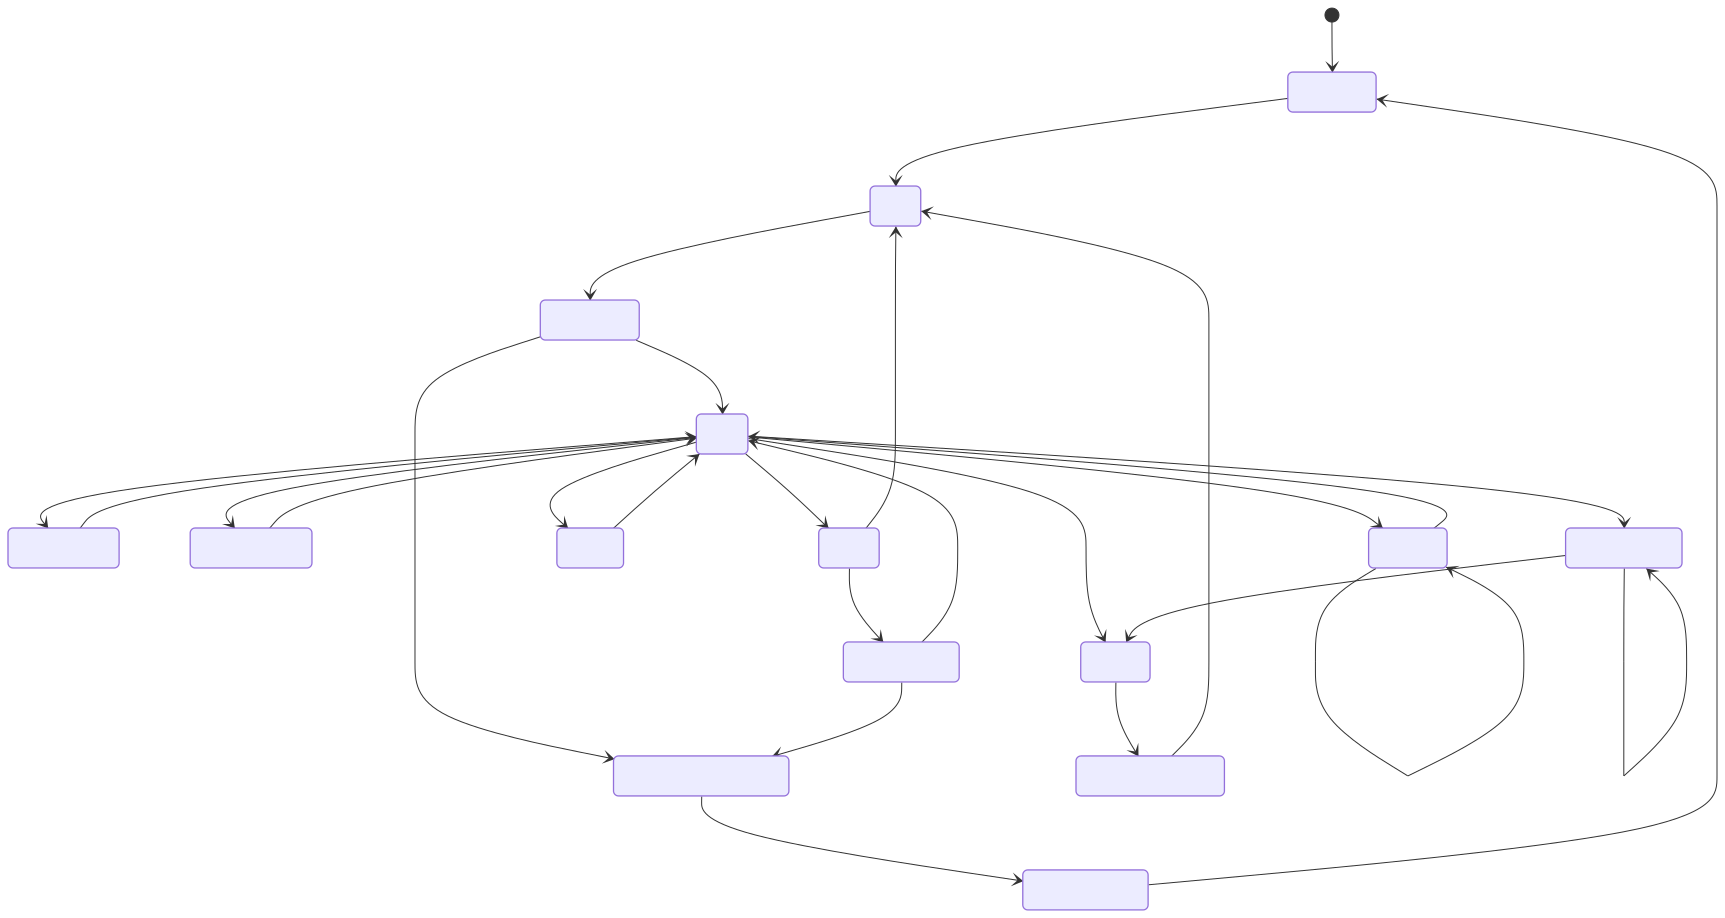
\includegraphics[width=1\textwidth]{fsm_diagram.png}
    \caption{Game Control FSM Diagram showing major state transitions.}
    \label{fig:fsm}
\end{figure}

\begin{table}[H]
    \centering
    \begin{tabular}{|l|l|}
    \hline
    \textbf{State} & \textbf{Description} \\ \hline
    \texttt{GEN} & Spawns a new tetromino from the randomizer. \\ \hline
    \texttt{IDLE} & Waits for user input (Left, Right, Rotate) or gravity timer. \\ \hline
    \texttt{MOVE\_*} & Updates x-coordinate. Checks collision; reverts if invalid. \\ \hline
    \texttt{ROTATE} & Tries standard rotation. If invalid, attempts Wall Kicks (SRS). \\ \hline
    \texttt{DOWN} & Moves piece down. If blocked, locks piece and goes to CLEAN. \\ \hline
    \texttt{CLEAN} & Scans for full rows, removes them, and shifts grid down. \\ \hline
    \texttt{HOLD} & Swaps current piece with held piece (if allowed). \\ \hline
    \texttt{GAME\_OVER} & Halts game until reset command is received. \\ \hline
    \end{tabular}
    \caption{Description of Main FSM States in \texttt{game\_control}.}
    \label{tab:fsm_states}
\end{table}

\subsubsection{Ghost Piece}
The `ghost\_calc` module continuously calculates where the current piece would land if dropped instantly. This "Ghost Piece" is rendered semi-transparently to aid player accuracy. Figure \ref{fig:drop_rot} shows the hardware logic for the drop and rotate operations.

\begin{figure}[H]
    \centering
    \includegraphics[width=0.8\textwidth]{Schematic/game_inst/drop_rot.png}
    \caption{Logic for piece manipulation (Drop and Rotate).}
    \label{fig:drop_rot}
\end{figure}

\subsection{Display Logic}
The display logic is decoupled from the game state update rate.
\begin{itemize}
    \item \textbf{CDC for Display}: The game state (field, current piece position) is transferred from the game domain to the pixel domain at the start of each frame (VSync) to ensure a tear-free image.
    \item \textbf{Rendering}: `draw\_tetris` calculates the color of the current pixel.
    \item \textbf{Sprites}: A ROM-based sprite system (`block\_sprite`) adds a beveled 3D look to the blocks. The sprites are stored as grayscale and tinted dynamically based on the piece type (e.g., Cyan for 'I', Purple for 'T').
\end{itemize}

\subsubsection{Sprite System Details}
The \texttt{block\_sprite} module stores a 16x16 pixel grayscale texture in ROM. Each pixel is a 12-bit value representing a brightness level. During rendering:
\begin{enumerate}
    \item The current pixel's position within a 32x32 block is calculated (using \texttt{curr\_x \% 32}).
    \item This address is sent to the sprite ROM, which returns a brightness value.
    \item The brightness is multiplied by a per-piece color (e.g., Cyan for I, Purple for T) to produce the final RGB output.
\end{enumerate}
This allows a single sprite texture to be reused for all 7 piece types, saving ROM space.

\begin{figure}[H]
    \centering
    \begin{subfigure}[b]{1.0\textwidth}
        \centering
        \includegraphics[width=\textwidth]{Schematic/draw_inst_pics/region_detectoin.png}
        \caption{Region Detection Logic (Stage 1)}
    \end{subfigure}
    \\
    \begin{subfigure}[b]{1.0\textwidth}
        \centering
        \includegraphics[width=\textwidth]{Schematic/draw_inst_pics/sprit_output.png}
        \caption{Sprite Output Logic (Stage 3)}
    \end{subfigure}
    \caption{Rendering Pipeline Implementation: Region detection determines the active object, while the sprite pipeline fetches pixel data.}
    \label{fig:draw_pipeline}
\end{figure}

\subsection{Game Logic Integration}
The game state is managed by the \texttt{game\_control} module. It handles:
\begin{itemize}
    \item \textbf{Gravity}: A counter generates a "tick" (approx 60Hz) to move pieces down.
    \item \textbf{Collisions}: The \texttt{check\_valid} module predicts next positions to prevent overlapping.
    \item \textbf{Ghost Piece}: We calculate where the piece would land if dropped instantly and render it semi-transparently.
\end{itemize}

\section{Testing and Verification}
We developed a comprehensive suite of testbenches to verify individual modules before integration. All simulations were run in Vivado XSim.

\subsection{Testbench Summary}
Table \ref{tab:tb_summary} lists the key testbenches and their verification targets.

\begin{table}[H]
    \centering
    \begin{tabular}{|l|l|c|}
    \hline
    \textbf{Testbench} & \textbf{Module Under Test} & \textbf{Result} \\ \hline
    \texttt{tb\_game\_control} & Core FSM (IDLE, MOVE, CLEAN) & 9/9 PASS \\ \hline
    \texttt{tb\_input\_manager} & DAS, one-shot logic & 17/17 PASS \\ \hline
    \texttt{tb\_rotate\_tetromino} & CW/CCW rotation matrix & 4/4 PASS \\ \hline
    \texttt{tb\_hold\_feature} & Hold swap, lockout & 9/9 PASS \\ \hline
    \texttt{tb\_generate\_tetromino} & 7-Bag randomizer & 13/13 PASS \\ \hline
    \texttt{tb\_vga\_out} & Sync pulse timing & Visual Pass \\ \hline
    \end{tabular}
    \caption{Summary of Testbenches and Results.}
    \label{tab:tb_summary}
\end{table}

\subsection{Game Control Simulation (\texttt{tb\_game\_control})}
The core FSM was verified by simulating key game scenarios: piece spawning, movement, rotation, hold functionality, and game over detection. Figure~\ref{fig:sim_waveform} shows a representative simulation waveform from Vivado XSim.

\begin{figure}[H]
    \centering
    \includegraphics[width=1.0\textwidth]{simulation_waveform.png}
    \caption{Simulation waveform from \texttt{tb\_game\_control} showing FSM state transitions, piece position updates, and control signals.}
    \label{fig:sim_waveform}
\end{figure}

\subsection{Input Manager Test (\texttt{tb\_input\_manager})}
This testbench verifies \textbf{DAS} (Delayed Auto Shift) and \textbf{one-shot} behavior. The log confirms that the rotation commands only fire once per key press, and the DAS repeat only triggers after a delay.

\begin{verbatim}
Test 1: Rotate CW One-Shot
  PASS: Rotate CW Triggered on press
  PASS: Rotate CW Pulse Ended after one cycle
  PASS: Rotate CW did not re-trigger while holding

Test 4: Left DAS (Delayed Auto Shift)
  PASS: Left Initial Move on press
  PASS: No trigger during DAS delay (15 frames)
  PASS: Left DAS Auto-Repeat Triggered
\end{verbatim}

\subsection{Rotation Test (\texttt{tb\_rotate\_tetromino})}
This testbench checks the basic matrix rotation (CW and CCW), ensuring the rotation index wraps correctly (e.g., $3 \rightarrow 0$ for CW).

\begin{verbatim}
Test 1: CW 0 -> 1
PASS: CW rotation 0 -> 1
Test 2: CW wrap 3 -> 0
PASS: CW rotation 3 -> 0
Test 3: CCW 0 -> 3
PASS: CCW rotation 0 -> 3
\end{verbatim}

\subsection{Hold Feature Test (\texttt{tb\_hold\_feature})}
This tests the swap-and-lockout mechanic. It verifies that after one hold, the player cannot hold again until a new piece has been placed.

\begin{verbatim}
Test 2: First Hold (Empty -> Store)
  Current piece before hold: J (1)
  After hold: curr=O, hold=J, hold_used=1
  PASS: First piece stored in hold

Test 3: Hold Lockout (Cannot Hold Twice Per Piece)
  Attempting second hold while hold_used=1...
  PASS: Lockout prevented second hold
\end{verbatim}

\subsection{Randomizer Test (\texttt{tb\_generate\_tetromino})}
Verified that the 7-Bag randomizer produces valid piece indices on sequential requests.

\begin{verbatim}
=== Test 2: Sequential Generation ===
PASS: Piece 0 - Valid index: 2
PASS: Piece 1 - Valid index: 2
...
PASS: Piece 9 - Valid index: 3
\end{verbatim}

\subsection{VGA Timing Test (\texttt{tb\_vga\_out})}
We ran a basic simulation over several frame periods to visually confirm that \texttt{hsync} and \texttt{vsync} pulsed at the expected intervals. The waveform was inspected to ensure \texttt{active\_area} was asserted only within the visible pixel range.

\subsection{Hardware Validation}
On the physical FPGA board (Nexys A7), we verified:
\begin{itemize}
    \item \textbf{Visual Output}: The Tetris grid is centered, block colors match type (Cyan I, Purple T), and the ghost piece renders correctly.
    \item \textbf{Input Response}: The DAS feels responsive, similar to official Tetris games.
    \item \textbf{Gameplay}: Full games were played through including line clears, reaching max level, game over, and reset functionality.
\end{itemize}

\section{References}

\begin{enumerate}

\item ``VESA Signal 1280 x 800 @ 60 Hz timing,'' tinyvga.com. [Online]. Available: \url{http://www.tinyvga.com/vga-timing/1280x800@60Hz}

\item ``Super Rotation System,'' TetrisWiki. [Online]. Available: \url{https://tetris.wiki/Super_Rotation_System}

\item ``Tetris Guideline,'' Hard Drop Tetris Wiki. [Online]. Available: \url{https://harddrop.com/wiki/Tetris_Guideline}

\item ``Random Generator,'' TetrisWiki. [Online]. Available: \url{https://tetris.wiki/Random_Generator}

\end{enumerate}

\section{Reflection}

This project provided invaluable hands-on experience in designing hardware systems from first principles to meet complex application requirements. The most significant technical skill gained was learning to architect hardware pipelines and finite state machines that operate across multiple clock domains, a challenge rarely encountered in pure software development but fundamental to digital design.

The video timing generation was particularly rewarding, as it offered concrete insight into how digital signals translate directly to visual information on a display. Implementing the 4-stage rendering pipeline and ensuring pixel-perfect synchronization with the VGA protocol deepened my understanding of hardware parallelism and real-time constraints.

Beyond clock domain crossing, the project presented substantial challenges in implementing smooth, responsive controls and the complex Super Rotation System with wall kicks and T-spin detection. Achieving fluid input handling required careful design of the Delayed Auto Shift (DAS) mechanism with dedicated hardware counters, while the SRS rotation system demanded implementing lookup tables and collision checking logic that could execute within tight timing constraints. Balancing game logic complexity with the need for deterministic, cycle-accurate behavior across multiple concurrent processes proved to be one of the most demanding aspects of the design.

If I were to approach this project again, I would invest more time upfront in formal verification of the FSM state transitions and create more comprehensive waveform-based testbenches for the rendering pipeline. While simulation testing caught most bugs, some visual artifacts only appeared during hardware deployment---earlier detection through more rigorous simulation could have saved debugging time on the physical FPGA.

Future enhancements to this implementation could include audio output using PWM for sound effects and background music, animated score displays with particle effects during line clears, and support for two-player competitive modes. Additionally, implementing variable DAS settings and customizable key mappings would improve the user experience for players with different skill levels and preferences.

\newpage
\appendix
\section{Appendix: Verilog Code}
This appendix contains the complete SystemVerilog source code for the AG Tetris project. Each file is prefaced with a brief description of its purpose.

% ==================== TOP LEVEL ====================
\subsection{Top Level Module}

\subsubsection*{game\_top.sv}
\textit{The main system integration module. It generates all required clock domains (83.46 MHz pixel, 50 MHz PS/2, 25 MHz game), instantiates all subsystems (VGA, input, game logic), and handles clock domain crossing between them.}
\lstinputlisting[language=Verilog]{game_top.sv}

% ==================== GLOBAL DEFINITIONS ====================
\subsection{Global Definitions}

\subsubsection*{GLOBAL.sv}
\textit{Shared header file containing game-wide constants such as grid dimensions (10$\times$20), tetromino type definitions, color indices, timing parameters, and custom data types used across all modules.}
\lstinputlisting[language=Verilog]{src/GLOBAL.sv}

% ==================== DISPLAY MODULES ====================
\subsection{Display Modules}

\subsubsection*{vga\_out.sv}
\textit{VGA timing generator. Produces horizontal/vertical sync pulses and active area signals for 1280$\times$800 resolution at 60 Hz. Outputs the current pixel coordinates (\texttt{curr\_x}, \texttt{curr\_y}) for the rendering pipeline.}
\lstinputlisting[language=Verilog]{src/display/vga_out.sv}

\subsubsection*{draw\_tetris.sv}
\textit{Main rendering engine. Implements a 4-stage pipeline to determine the color of each pixel by checking if it falls within the game grid, next piece preview, hold area, score display, or UI borders.}
\lstinputlisting[language=Verilog]{src/display/draw_tetris.sv}

\subsubsection*{block\_sprite.sv}
\textit{Sprite ROM for tetromino blocks. Stores a 16$\times$16 grayscale texture that is tinted with per-piece colors during rendering to give blocks a beveled 3D appearance.}
\lstinputlisting[language=Verilog]{src/display/block_sprite.sv}

\subsubsection*{draw\_number.sv}
\textit{Numeric digit renderer. Draws score and level numbers on screen by mapping digit values to a font ROM and outputting pixel data.}
\lstinputlisting[language=Verilog]{src/display/draw_number.sv}

\subsubsection*{draw\_string.sv}
\textit{Text string renderer. Draws static text labels ("SCORE", "LEVEL", "NEXT", "HOLD") on the game UI using a character ROM.}
\lstinputlisting[language=Verilog]{src/display/draw_string.sv}

\subsubsection*{seg7\_key\_display.sv}
\textit{7-segment display driver. Shows debug information (current key code, game state) on the FPGA board's 8-digit 7-segment display using time-multiplexed digit scanning.}
\lstinputlisting[language=Verilog]{src/display/seg7_key_display.sv}

% ==================== LOGIC MODULES ====================
\subsection{Game Logic Modules}

\subsubsection*{game\_control.sv}
\textit{Central game state machine. Implements the main FSM with 15 states governing piece spawning, movement, rotation (with SRS wall kicks), gravity, line clearing, hold functionality, and game over detection.}
\lstinputlisting[language=Verilog]{src/logic/game_control.sv}

\subsubsection*{generate\_tetromino.sv}
\textit{7-Bag randomizer. Generates tetromino pieces using the standard 7-bag algorithm, ensuring all 7 piece types appear exactly once before repeating.}
\lstinputlisting[language=Verilog]{src/logic/generate_tetromino.sv}

\subsubsection*{check\_valid.sv}
\textit{Collision detection. Checks if a proposed piece position is valid by testing for collisions with the field boundaries and locked blocks.}
\lstinputlisting[language=Verilog]{src/logic/check_valid.sv}

\subsubsection*{clean\_field.sv}
\textit{Line clearing logic. Detects complete rows, removes them, shifts all rows above downward, and returns the count of lines cleared for scoring.}
\lstinputlisting[language=Verilog]{src/logic/clean_field.sv}

\subsubsection*{create\_field.sv}
\textit{Field manipulation helper. Merges the current falling piece into the game field array when it locks in place.}
\lstinputlisting[language=Verilog]{src/logic/create_field.sv}

\subsubsection*{rotate\_tetromino.sv}
\textit{Rotation with wall kicks. Implements the Super Rotation System (SRS) by attempting standard rotation first, then trying up to 4 alternative kick offsets if collision occurs.}
\lstinputlisting[language=Verilog]{src/logic/rotate_tertomino.sv}

\subsubsection*{rotate\_clockwise.sv}
\textit{Basic rotation matrix. Performs a simple 90-degree clockwise rotation of a 4$\times$4 tetromino shape matrix.}
\lstinputlisting[language=Verilog]{src/logic/rotate_clockwise.sv}

\subsubsection*{ghost\_calc.sv}
\textit{Ghost piece calculator. Projects the current piece downward to find where it would land, enabling the semi-transparent "ghost" preview.}
\lstinputlisting[language=Verilog]{src/logic/ghost_calc.sv}

\subsubsection*{spin\_detector.sv}
\textit{T-Spin detection. Checks the 3-corner rule after T-piece rotations to determine if a T-Spin occurred for bonus scoring.}
\lstinputlisting[language=Verilog]{src/logic/spin_detector.sv}

\subsubsection*{bin\_to\_bcd.sv}
\textit{Binary to BCD converter. Converts binary score values to Binary-Coded Decimal for display on the 7-segment display.}
\lstinputlisting[language=Verilog]{src/logic/bin_to_bcd.sv}

% ==================== INPUT MODULES ====================
\subsection{Input Processing Modules}

\subsubsection*{ps2\_keyboard.sv}
\textit{PS/2 keyboard decoder. Processes raw scan codes from PS2Receiver, handles make/break prefixes (0xF0) and extended codes (0xE0), and outputs key events.}
\lstinputlisting[language=Verilog]{src/input/ps2_keyboard.sv}

\subsubsection*{PS2Receiver.sv}
\textit{Low-level PS/2 protocol handler. Samples the PS/2 clock and data lines to deserialize 11-bit frames (start, 8 data, parity, stop) into raw scan codes.}
\lstinputlisting[language=Verilog]{src/input/PS2Receiver.sv}

\subsubsection*{input\_manager.sv}
\textit{Input processing with DAS. Implements Delayed Auto Shift for smooth left/right movement and one-shot behavior for rotation, drop, and hold commands.}
\lstinputlisting[language=Verilog]{src/input/input_manager.sv}

\subsubsection*{debouncer.sv}
\textit{Button debouncer. Removes mechanical bounce from physical push-button inputs using a shift register and stability counter.}
\lstinputlisting[language=Verilog]{src/input/debouncer.sv}

% ==================== TESTBENCHES ====================
\subsection{Testbenches and Simulation Logs}

\subsubsection*{tb\_game\_control.sv}
\textit{Core FSM testbench. Verifies piece spawning, movement, rotation, hold functionality, hard drop, ghost position, and game over detection.}
\lstinputlisting[language=Verilog]{test/tb_game_control.sv}
\textbf{Simulation Log:}
\lstinputlisting[language={}]{test_logs/tb_game_control.log}

\subsubsection*{tb\_input\_manager.sv}
\textit{Input processing testbench. Tests Delayed Auto Shift (DAS) timing and one-shot behavior for rotation, drop, and hold commands.}
\lstinputlisting[language=Verilog]{test/tb_input_manager.sv}
\textbf{Simulation Log:}
\lstinputlisting[language={}]{test_logs/tb_input_manager.log}

\subsubsection*{tb\_rotate\_tetromino.sv}
\textit{Rotation testbench. Verifies clockwise and counter-clockwise rotation with SRS wall kick logic.}
\lstinputlisting[language=Verilog]{test/tb_rotate_tetromino.sv}
\textbf{Simulation Log:}
\lstinputlisting[language={}]{test_logs/tb_rotate_tertomino.log}

\subsubsection*{tb\_hold\_feature.sv}
\textit{Hold mechanic testbench. Tests piece swapping, hold lockout (preventing double-hold per piece), and edge cases.}
\lstinputlisting[language=Verilog]{test/tb_hold_feature.sv}
\textbf{Simulation Log:}
\lstinputlisting[language={}]{test_logs/tb_hold_feature.log}

\subsubsection*{tb\_generate\_tetromino.sv}
\textit{7-Bag randomizer testbench. Verifies that pieces are generated in valid range and follow the 7-bag algorithm.}
\lstinputlisting[language=Verilog]{test/tb_generate_tetromino.sv}
\textbf{Simulation Log:}
\lstinputlisting[language={}]{test_logs/tb_generate_teromino.log}

\subsubsection*{tb\_vga\_out.sv}
\textit{VGA timing testbench. Runs simulation over multiple frames to verify hsync, vsync, and active\_area signals.}
\lstinputlisting[language=Verilog]{test/tb_vga_out.sv}
\textbf{Simulation Log:}
\lstinputlisting[language={}]{test_logs/tb_vga.log}

\subsubsection*{tb\_ps2\_keyboard.sv}
\textit{PS/2 decoder testbench. Tests scan code processing including make/break detection and extended key codes.}
\lstinputlisting[language=Verilog]{test/tb_ps2_keyboard.sv}
\textbf{Simulation Log:}
\lstinputlisting[language={}]{test_logs/tb_ps2_keyboard.log}

\subsubsection*{tb\_PS2Receiver.sv}
\textit{Low-level PS/2 testbench. Verifies bit-level deserialization of PS/2 clock and data signals.}
\lstinputlisting[language=Verilog]{test/tb_PS2Receiver.sv}
\textbf{Simulation Log:}
\lstinputlisting[language={}]{test_logs/tb_PS2Receiver.log}

\end{document}
